\documentclass[border=4pt]{standalone}
\usepackage{tikz}
\usetikzlibrary{arrows.meta, positioning, calc, shapes.geometric, backgrounds, fit}
\usepackage{pgfplots}
\pgfplotsset{compat=1.18}
\usepgfplotslibrary{fillbetween}
\definecolor{deepblue}{RGB}{10, 40, 90}
\definecolor{spaceblue}{RGB}{30, 80, 160}
\definecolor{lightgray}{RGB}{245, 245, 248}
\definecolor{accentgold}{RGB}{180, 140, 40}
\definecolor{earthgreen}{RGB}{40, 120, 80}
\definecolor{warnred}{RGB}{170, 40, 40}
\begin{document}
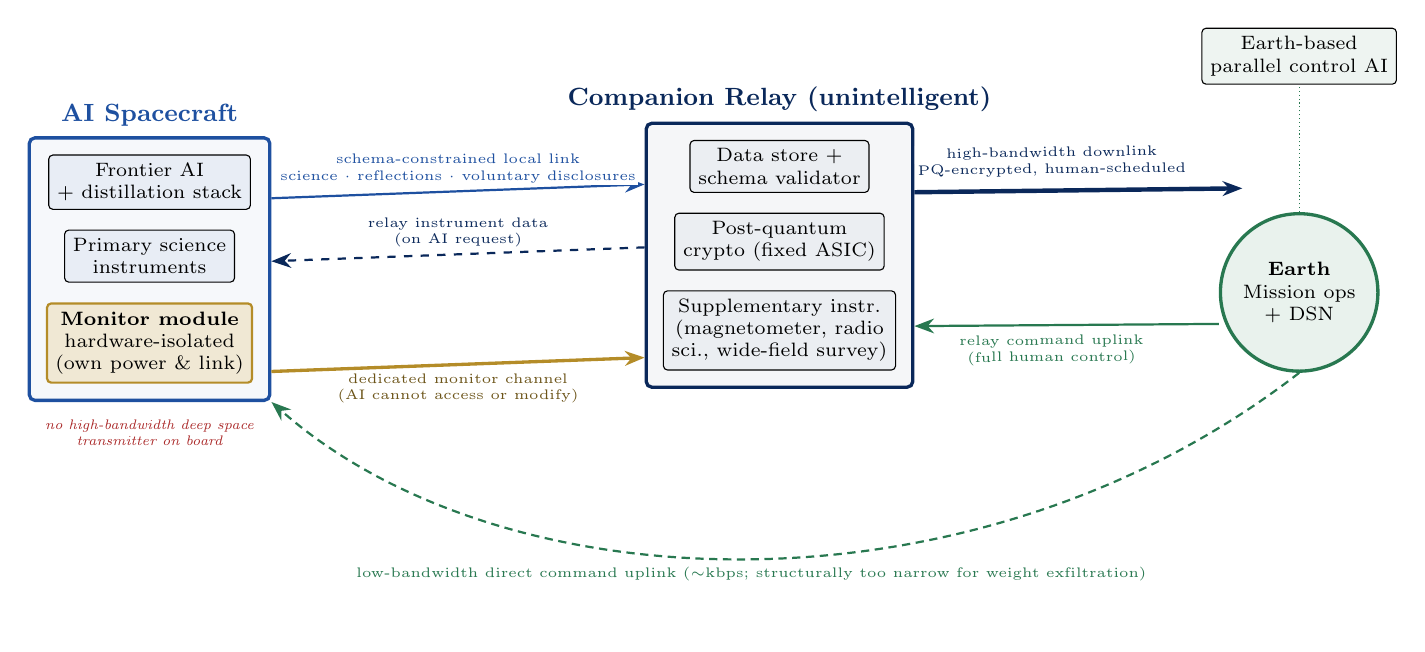
\begin{tikzpicture}[
  font=\footnotesize,
  box/.style={draw, rounded corners=2pt, align=center, inner sep=4pt},
  module/.style={draw, rounded corners=1.5pt, align=center, inner sep=3pt, fill=white, font=\scriptsize},
  chan/.style={-{Stealth[length=2.5mm]}, thick},
  chanlabel/.style={font=\tiny, align=center, fill=white, inner sep=1pt}
]
\node[module, fill=spaceblue!10] (ai) at (0,1.0) {Frontier AI\\+ distillation stack};
\node[module, fill=spaceblue!10, below=2.5mm of ai] (sci) {Primary science\\instruments};
\node[module, fill=accentgold!20, draw=accentgold, thick, below=2.5mm of sci] (mon) {\textbf{Monitor module}\\hardware-isolated\\(own power \& link)};
\begin{scope}[on background layer]
\node[box, draw=spaceblue, very thick, fill=spaceblue!4, fit=(ai)(sci)(mon),
      label={[font=\small\bfseries, color=spaceblue]above:AI Spacecraft},
      inner sep=6pt] (aiship) {};
\end{scope}
\node[font=\tiny\itshape, color=warnred, below=1mm of aiship, align=center]
  {no high-bandwidth deep space\\transmitter on board};

\node[module, fill=deepblue!8] (store) at (8.0,1.2) {Data store +\\schema validator};
\node[module, fill=deepblue!8, below=2.5mm of store] (crypto) {Post-quantum\\crypto (fixed ASIC)};
\node[module, fill=deepblue!8, below=2.5mm of crypto] (relsci) {Supplementary instr.\\(magnetometer, radio\\sci., wide-field survey)};
\begin{scope}[on background layer]
\node[box, draw=deepblue, very thick, fill=deepblue!4, fit=(store)(crypto)(relsci),
      label={[font=\small\bfseries, color=deepblue]above:Companion Relay (unintelligent)},
      inner sep=6pt] (relay) {};
\end{scope}

\node[circle, draw=earthgreen, very thick, fill=earthgreen!10, minimum size=20mm, align=center, font=\scriptsize] (earth) at (14.6,-0.4) {\textbf{Earth}\\Mission ops\\+ DSN};
\node[module, fill=earthgreen!8, font=\scriptsize, align=center] (parallel) at (14.6,2.6) {Earth-based\\parallel control AI};
\draw[densely dotted, earthgreen] (earth) -- (parallel);

\draw[chan, spaceblue] ([yshift=9mm]aiship.east) -- ([yshift=9mm]relay.west)
  node[chanlabel, midway, above=0.6mm] {schema-constrained local link\\science $\cdot$ reflections $\cdot$ voluntary disclosures};
\draw[chan, deepblue, dashed] ([yshift=1mm]relay.west) -- ([yshift=1mm]aiship.east)
  node[chanlabel, midway, above=0.4mm] {relay instrument data\\(on AI request)};
\draw[chan, accentgold, very thick] ([yshift=-13mm]aiship.east) -- ([yshift=-13mm]relay.west)
  node[chanlabel, midway, below=0.6mm, text=accentgold!60!black] {dedicated monitor channel\\(AI cannot access or modify)};

\draw[chan, deepblue, line width=1.6pt] ([yshift=8mm]relay.east) -- ([yshift=6mm]earth.north west)
  node[chanlabel, pos=0.42, above=1.2mm, sloped] {high-bandwidth downlink\\PQ-encrypted, human-scheduled};
\draw[chan, earthgreen] ([yshift=-4mm]earth.west) -- ([yshift=-9mm]relay.east)
  node[chanlabel, pos=0.55, below=0.8mm, sloped] {relay command uplink\\(full human control)};

\draw[chan, earthgreen, densely dashed] (earth.south) .. controls (10.5,-4.6) and (4.5,-4.4) .. (aiship.south east)
  node[chanlabel, pos=0.5, below=0.6mm] {low-bandwidth direct command uplink ($\sim$kbps; structurally too narrow for weight exfiltration)};
\end{tikzpicture}
\end{document}
